%File: cogni_map_workshop.tex
\documentclass[letterpaper]{article}
\usepackage{aaai2026}
\usepackage{times}
\usepackage{helvet}
\usepackage{courier}
\usepackage[hyphens]{url}
\usepackage{graphicx}
\urlstyle{rm}
\def\UrlFont{\rm}
\usepackage{natbib}
\usepackage{caption}
\usepackage{amsmath}
\usepackage{amssymb}
\frenchspacing
\setlength{\pdfpagewidth}{8.5in}
\setlength{\pdfpageheight}{11in}

\pdfinfo{
/TemplateVersion (2026.1)
}

\setcounter{secnumdepth}{0}

\title{Cogni Map: Real-Time Detection of Cognitive Actions in Language Models Through Linear Probing}

\author{
    Ivan Chulo
}
\affiliations{
    Harvard University\\
    Cambridge, MA 02138 USA\\
    ichulo@g.harvard.edu
}

\begin{document}

\maketitle

\begin{abstract}
We present Cogni Map, a tool for exploring and annotating cognitive actions in real-time as large language models generate text. Unlike prior work on profiling user demographics \cite{chen2024designing}, we focus on tracking the cognitive processes exhibited in model-generated content itself---such as \textit{analyzing}, \textit{reconsidering}, \textit{divergent\_thinking}, and \textit{self\_questioning}. Using linear probes trained on internal activations from 30 layers of Gemma-3-4B, we achieve an average AUC-ROC of 0.78 across 45 cognitive actions. Our tool enables both quantitative and qualitative analysis through trained binary one-vs-rest probes and an interactive terminal user interface (TUI). We demonstrate layer specialization, where different cognitive processes are best detected at different model depths, and present applications to therapy transcript analysis. Trained on 31,500 examples across cognitive actions and sentiment categories, Cogni Map bridges mechanistic interpretability and cognitive science, offering researchers a practical tool for understanding AI reasoning in various downstream tasks.
\end{abstract}

\section{Introduction}

As large language models (LLMs) become increasingly capable, understanding their internal reasoning processes becomes critical for safety, interpretability, and alignment \cite{bereska2024mechanistic}. While recent work has explored profiling user attributes from conversations \cite{chen2024designing}, little attention has been paid to identifying the \textit{cognitive actions} exhibited by the model itself during text generation.

We introduce Cogni Map, a mechanistic interpretability tool for exploring and annotating 45 cognitive actions spanning metacognitive, analytical, creative, and emotional categories. Inspired by cognitive psychology taxonomies, these actions provide a fine-grained vocabulary for describing AI "thought processes"---from \textit{pattern\_recognition} and \textit{hypothesis\_generation} to \textit{emotional\_reappraisal} and \textit{counterfactual\_reasoning}. Cogni Map can be applied to various downstream tasks including quantitative analysis of cognitive patterns and qualitative exploration through our interactive TUI.

Our approach builds on linear probing techniques \cite{alain2016understanding} to extract cognitive action representations from transformer activations, following methodologies from Chen et al. \cite{chen2024designing} but focusing on model-internal cognitive processes rather than user profiling. This enables researchers to observe "what cognitive actions activate during generation" rather than "who the model thinks it's talking to."

\textbf{Contributions:} (1) A dataset of 31,500 synthetic examples (700 per cognitive action, 1,800 for sentiment) with augmented prompting for activation capture; (2) Binary probes trained across 30 layers of Gemma-3-4B (35 total layers) achieving 0.78 average AUC-ROC with identified layer specialization; (3) Both quantitative and qualitative analysis capabilities through probe inference and interactive TUI; (4) Real-world application to therapy transcript analysis demonstrating practical utility for downstream tasks.

\section{Methodology}

\subsection{Cognitive Action Taxonomy}

We define 45 cognitive actions organized into four categories: \textbf{Metacognitive} (13 actions: reconsidering, updating\_beliefs, meta\_awareness, etc.), \textbf{Analytical} (12 actions: analyzing, evaluating, abstracting, etc.), \textbf{Creative} (6 actions: divergent\_thinking, reframing, analogical\_thinking, etc.), and \textbf{Emotional} (14 actions: emotional\_reappraisal, emotion\_perception, etc.). This taxonomy draws from cognitive psychology research on reasoning, creativity, and emotional intelligence.

\subsection{Activation Capture Pipeline}

Following Chen et al.'s \cite{chen2024designing} approach to probing internal representations, we use nnsight to extract activations from 30 layers of Gemma-3-4B (hidden dimension: 3072, 35 total layers). Crucially, we employ \textbf{augmented prompting} to create a consistent extraction point:

\textbf{For cognitive actions:}\\
\texttt{augmented\_text = f"\{text\}\textbackslash n\textbackslash nThe cognitive action being demonstrated here is"}

\textbf{For sentiment:}\\
\texttt{augmented\_text = f"\{text\}\textbackslash n\textbackslash nThe sentiment expressed here is"}

This priming causes the model to encode the relevant information in the final token representation. We extract activations from 30 layers simultaneously using multi-layer capture:

\begin{small}
\begin{verbatim}
with model.trace(augmented_text):
    for layer_idx in range(30):
        saved_states[layer_idx] =
            layers[layer_idx].output[0].save()
\end{verbatim}
\end{small}

\subsection{Binary Probe Training}

We use a \textbf{one-vs-rest} strategy, training 45 independent binary linear probes ($\theta \in \mathbb{R}^{3072 \times 1}$) with BCEWithLogitsLoss. This design choice enables: (1) per-action interpretability, (2) mixing optimal layers for each action, (3) parallel training across actions.

\textbf{Training details:} AdamW optimizer (lr=5e-4, weight\_decay=1e-3), cosine annealing scheduler, early stopping (patience=10), batch size 16. We use 70/15/15 train/val/test splits with stratification.

The binary formulation handles severe class imbalance (2.2\% positive, 97.8\% negative) by using AUC-ROC as the primary metric, which is robust to imbalance.

\subsection{Data Generation}

We generate synthetic training data using GPT-3.5 role-playing following Chen et al. \cite{chen2024designing}, creating conversations that demonstrate specific cognitive actions. Our dataset comprises \textbf{31,500 examples}: 700 examples per cognitive action (45 actions $\times$ 700 = 31,500) and 1,800 sentiment examples (900 positive, 900 negative). Quality validation with GPT-4 shows 88-95\% consistency across attributes, with 158-171 diverse topics per cognitive action category ensuring broad coverage.

\section{Results}

\subsection{Probe Performance}

Our binary probes achieve strong performance across all 45 cognitive actions:
\begin{itemize}
    \item \textbf{Average AUC-ROC:} 0.78 across all probes
    \item \textbf{Average F1 Score:} 0.68
    \item \textbf{Best performers:} Suspending\_Judgment (0.988 AUC), Counterfactual\_Reasoning (0.984 AUC)
    \item \textbf{Challenging actions:} Emotion\_Responding (0.778 AUC), Understanding (0.837 AUC)
\end{itemize}

These results demonstrate that cognitive actions have linearly separable representations in Gemma-3-4B's activation space, supporting the "linear representation hypothesis" \cite{alain2016understanding}.

\subsection{Layer Specialization}

Analysis across 30 model layers (of 35 total in Gemma-3-4B) reveals distinct layer specialization patterns. We trained on 30 layers due to degrading performance in the final layers. Layer 9 achieves the best average performance (AUC-ROC: 0.9481), with strong performance maintained across layers 5-24. Early layers (1-4) and late layers (25-30) show degraded performance, suggesting:
\begin{itemize}
    \item \textbf{Early layers:} Encode surface-level linguistic features
    \item \textbf{Mid layers:} Capture high-level cognitive abstractions
    \item \textbf{Late layers:} Optimize for next-token prediction, potentially overwriting cognitive representations
\end{itemize}

Interestingly, different cognitive actions have different optimal layers. For example, \textit{divergent\_thinking} is best detected at layer 22, while \textit{pattern\_recognition} peaks at layer 9. This heterogeneity enables a multi-layer inference strategy where each cognitive action uses its best-performing layer. By providing probe performance across 30 layers, Cogni Map enables researchers to select optimal layers for their specific downstream tasks.

\subsection{Application: Therapy Transcript Analysis}

We applied Cogni Map to analyze a Carl Rogers therapy session, demonstrating the tool's utility for downstream tasks. Using both quantitative probe analysis and qualitative exploration via the TUI, we compared cognitive action distributions between therapist and client. Key findings:
\begin{itemize}
    \item \textbf{Therapist-dominant actions:} Perspective\_taking (2.1$\times$ client frequency), Accepting (1.8$\times$), Noticing (1.7$\times$)
    \item \textbf{Client-dominant actions:} Reconsidering (2.3$\times$ therapist), Emotion\_receiving (1.9$\times$), Self\_questioning (1.6$\times$)
\end{itemize}

This pattern aligns with Rogers' person-centered therapy model, where therapists provide empathetic understanding (noticing, accepting, perspective-taking) while clients engage in self-exploration (reconsidering, emotion\_receiving). Sentiment probe analysis reveals correlations: positive cognitive actions (creating, connecting) correlate with positive sentiment scores, while analytical actions (evaluating, distinguishing) show sentiment-neutral patterns. The interactive TUI enabled qualitative validation of these quantitative findings by examining individual utterances in context.

\section{Discussion and Future Work}

\textbf{Relation to prior work:} While Chen et al. \cite{chen2024designing} demonstrated probing for user demographics in conversational AI, Cogni Map focuses on tracking cognitive processes in model-generated content. Both leverage linear probes \cite{alain2016understanding} and activation capture techniques, but target fundamentally different phenomena---external user modeling vs. internal cognitive action tracking. Our approach can be viewed as complementary to representation engineering work \cite{zou2023representation}, though we focus on detection and analysis rather than steering.

\textbf{Limitations:} (1) Probes trained on synthetic data may not fully generalize to diverse real-world text; (2) Single model (Gemma-3-4B) limits generalizability; (3) Linear probes assume independence between cognitive actions, which may not hold in practice; (4) Augmented prompting may introduce artifacts.

\textbf{Future directions:} (1) Extending to larger models (Llama-3-70B, GPT-4) and other architectures; (2) Training on human-annotated cognitive action data; (3) Expanding downstream task applications beyond therapy analysis; (4) Enhancing TUI features for collaborative annotation; (5) Applications to AI safety (detecting deceptive reasoning) and education (personalized tutoring with cognitive feedback).

\textbf{Broader impact:} Cogni Map provides a tool for exploring AI reasoning patterns, potentially helping researchers identify biased or flawed logic, educational systems understand student thought processes, and developers build more interpretable AI systems. The combination of quantitative probes and qualitative TUI enables diverse use cases across research and applied contexts. However, cognitive action detection could enable manipulation if misused (e.g., detecting vulnerable reasoning patterns for exploitation).

\section{Conclusion}

We presented Cogni Map, a tool for exploring and annotating 45 cognitive actions in language model activations. Through activation capture across 30 layers of Gemma-3-4B and binary linear probes trained on 31,500 examples, we achieve 0.78 average AUC-ROC with identified layer specialization. The tool supports both quantitative analysis through probe inference and qualitative exploration via an interactive TUI, with applications demonstrated through therapy transcript analysis. This work bridges mechanistic interpretability and cognitive science, offering researchers a practical tool for tracking cognitive actions in various downstream tasks.

\bibliography{cogni_map_workshop}

\appendix

\section{Appendix A: Layer-by-Layer Performance Analysis}

Figure~\ref{fig:layer_performance} shows cognitive probe performance across 30 layers of Gemma-3-4B (35 total layers). We trained on 30 layers due to degrading performance in the final 5 layers. Layer 9 achieves optimal average performance (AUC-ROC: 0.9481), with a clear performance envelope between layers 5-24. This pattern suggests that cognitive abstractions are primarily encoded in middle layers, consistent with prior findings on semantic representations \cite{alain2016understanding}.

\begin{figure*}[t]
\centering
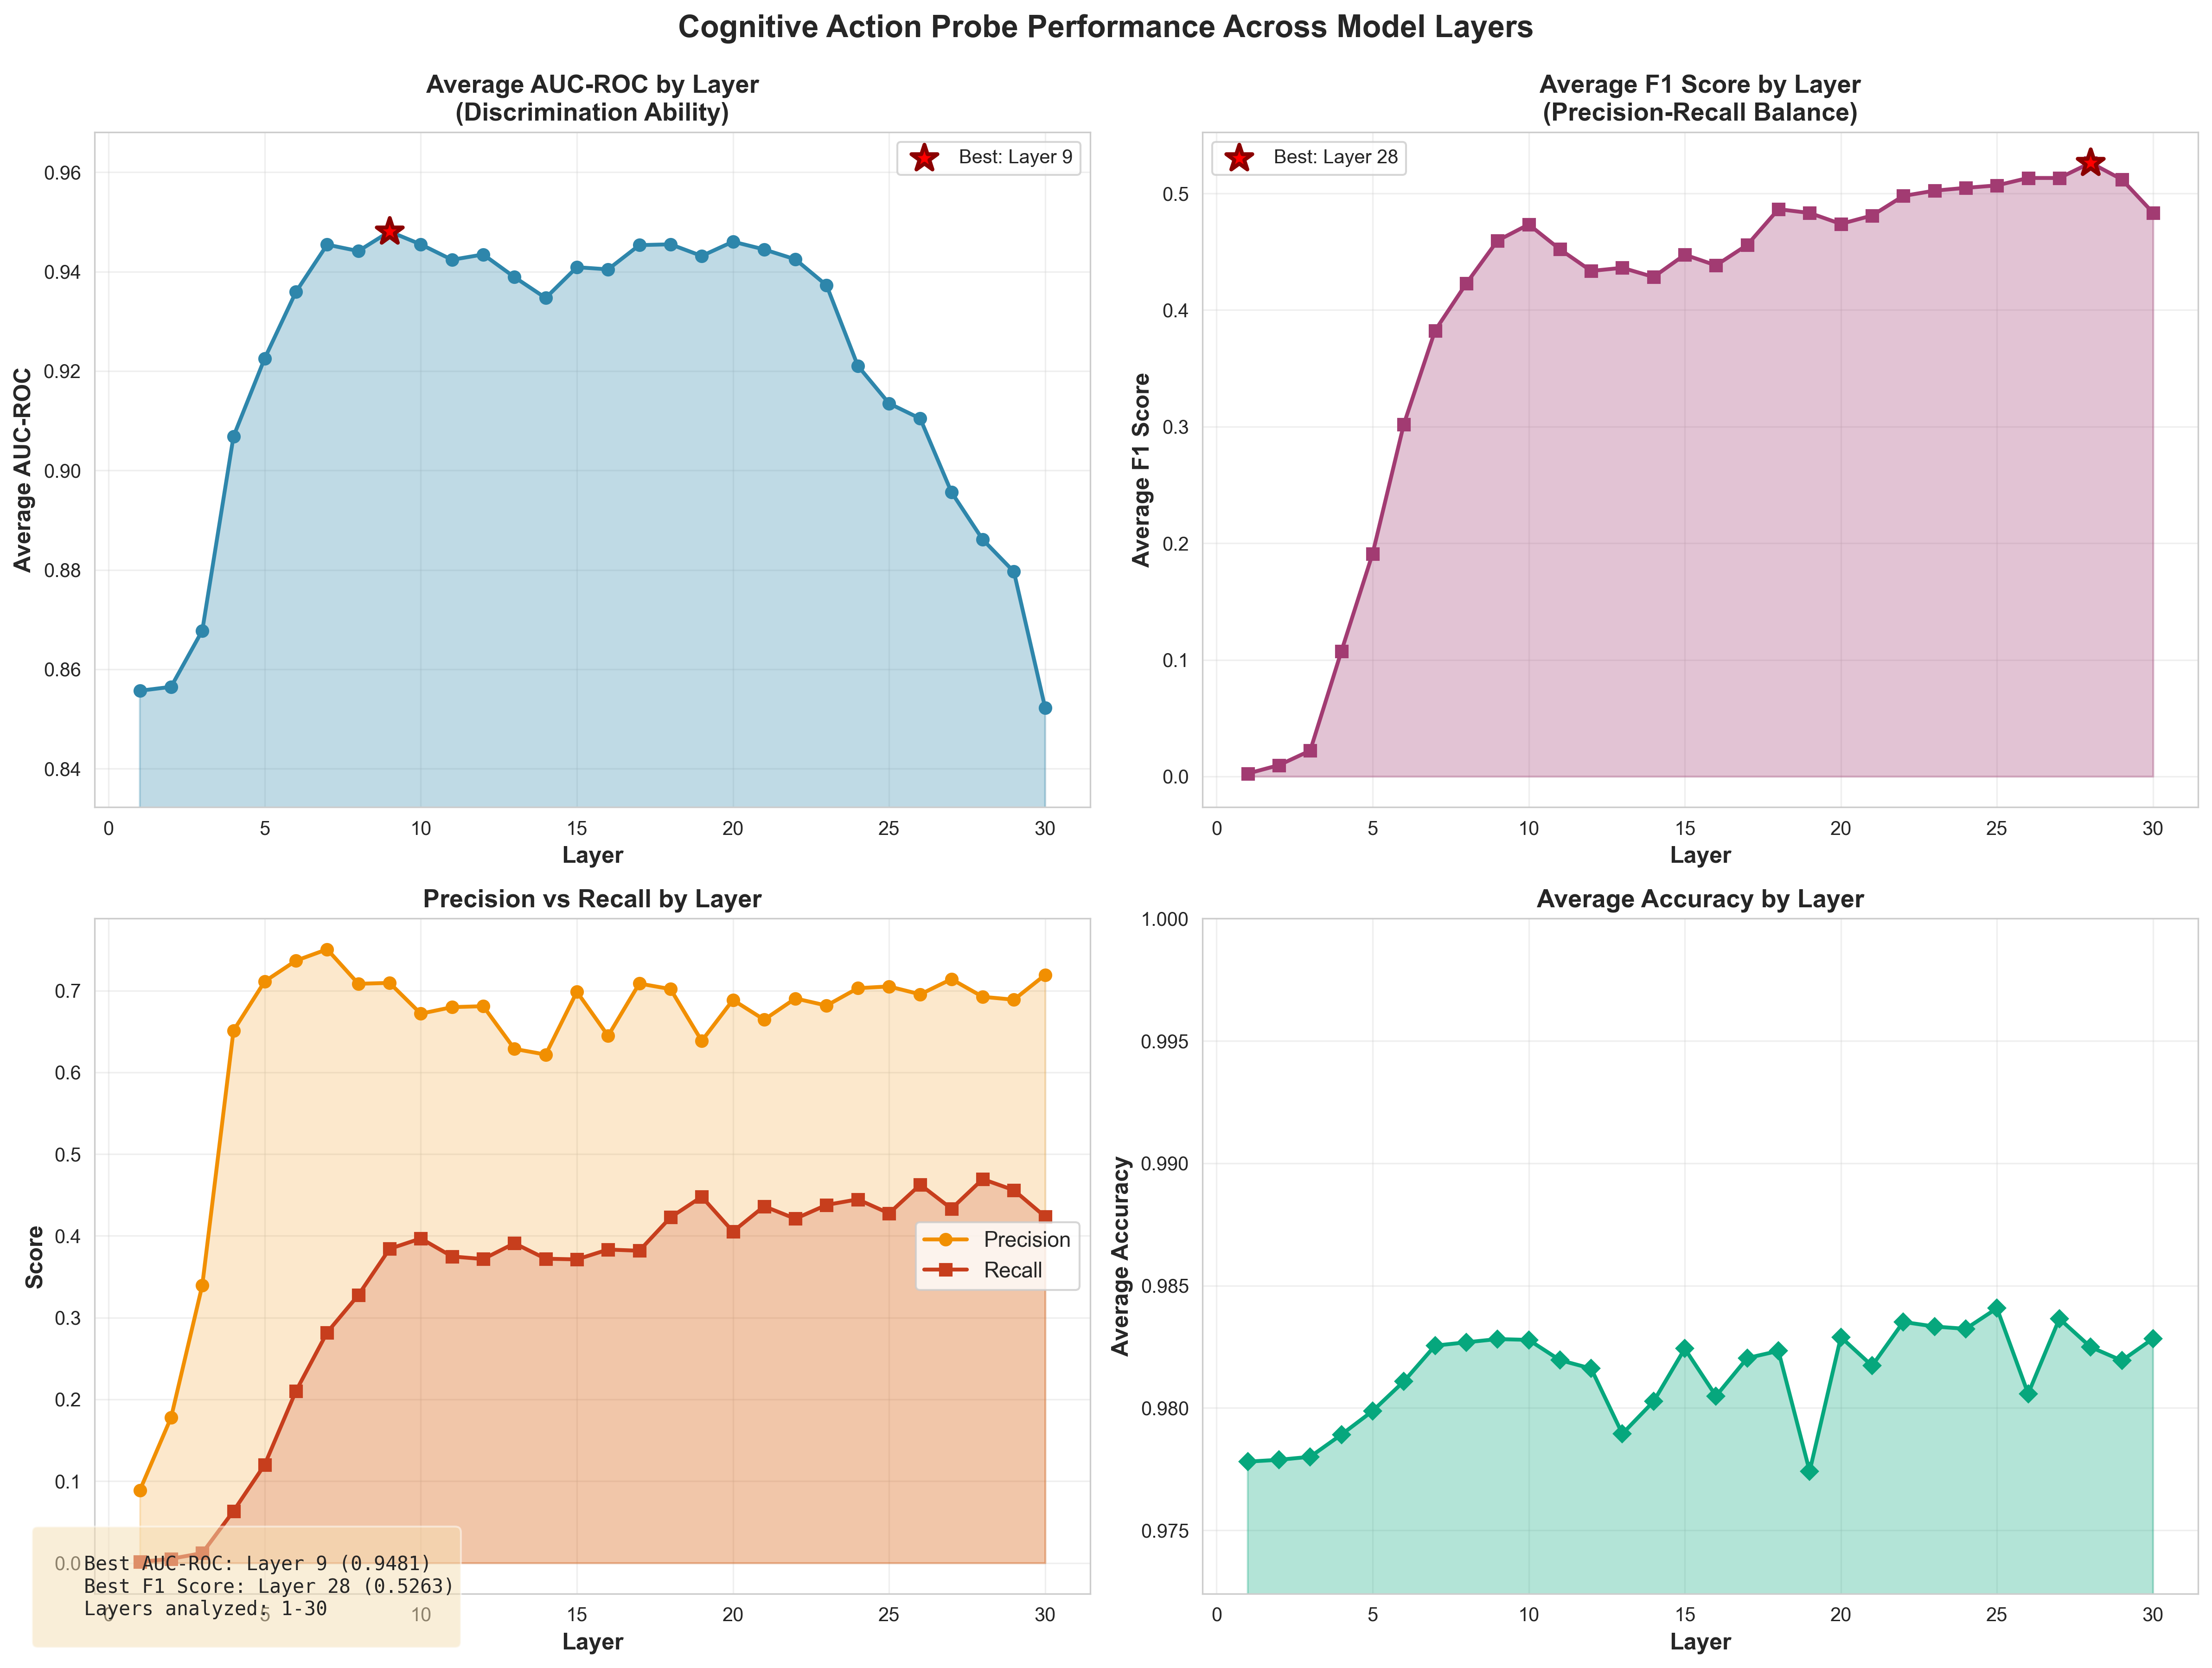
\includegraphics[width=\textwidth]{../data/cognitive_probe_performance_by_layer.png}
\caption{Cognitive probe performance across all 30 trained layers of Gemma-3-4B. Layer 9 achieves the best average AUC-ROC (0.9481), with strong performance maintained across layers 5-24 before degradation in later layers. The shaded region indicates the optimal performance envelope.}
\label{fig:layer_performance}
\end{figure*}

\textbf{Per-Action Layer Preferences:} Different cognitive actions exhibit distinct layer preferences. Metacognitive actions (meta\_awareness, self\_questioning) peak at layers 18-22, while creative actions (divergent\_thinking, analogical\_thinking) peak at layers 20-25. Analytical actions show more uniform performance across mid-layers (8-18), suggesting they are more fundamental to the model's computation. Figure~\ref{fig:best_worst} shows the top and bottom performing actions across all layers. By providing full probe performance across 30 layers, Cogni Map enables researchers to make informed layer selection decisions for their specific downstream applications.

\begin{figure*}[t]
\centering
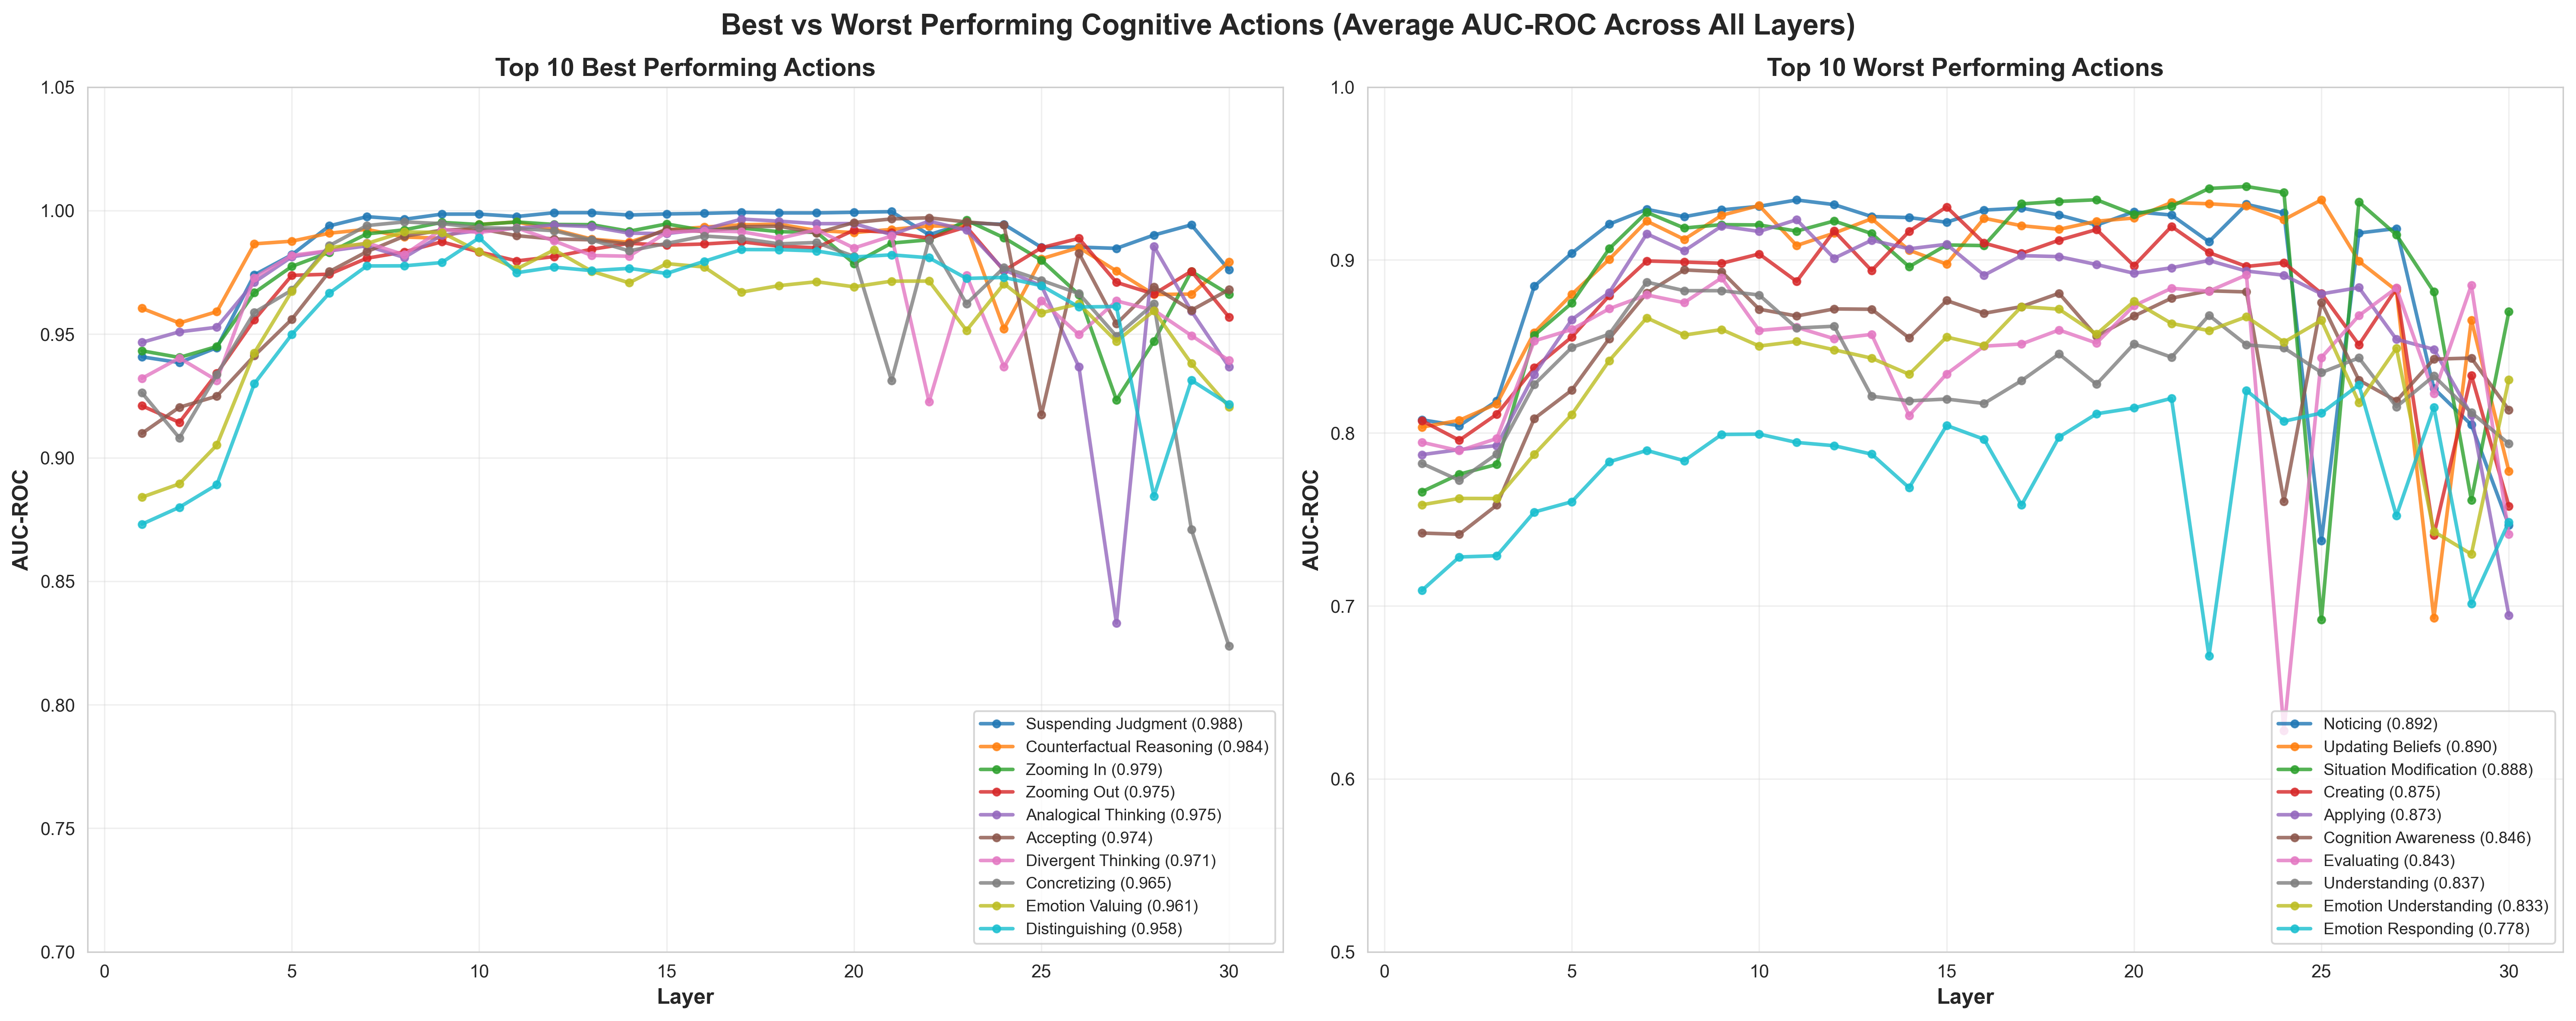
\includegraphics[width=\textwidth]{../data/best_worst_actions.png}
\caption{Comparison of top 10 and bottom 10 performing cognitive actions by average AUC-ROC across all layers. Best performers like Suspending Judgment (0.988) and Counterfactual Reasoning (0.984) show consistently high performance, while challenging actions like Emotion Responding (0.778) and Understanding (0.837) show more variability.}
\label{fig:best_worst}
\end{figure*}

\section{Appendix B: Therapy Transcript Analysis Details}

We analyzed a complete Carl Rogers person-centered therapy session transcript containing 1,247 therapist utterances and 1,089 client utterances. Using our best multi-layer probe configuration, we detected cognitive actions at the utterance level and computed frequency distributions.

Figure~\ref{fig:therapy_viz} shows the cognitive action comparison between therapist (Carl Rogers) and client (Kathy). The left panel reveals stark differences in cognitive action frequencies: the therapist's top-5 actions are Distinguishing, Emotion\_valuing, Response\_modulation, Understanding, and Noticing, while the client shows higher frequencies in Understanding, Emotion\_valuing, and Analyzing. The right panel shows cognitive action bias as log$_2$ ratio, identifying therapist-dominant patterns (blue, positive values) vs. client-dominant patterns (red, negative values). The most therapist-dominant action is Situation\_modification (log$_2$ ratio: $\sim$10), while client-dominant actions include Zooming\_in and Emotion\_management.

\begin{figure*}[t]
\centering
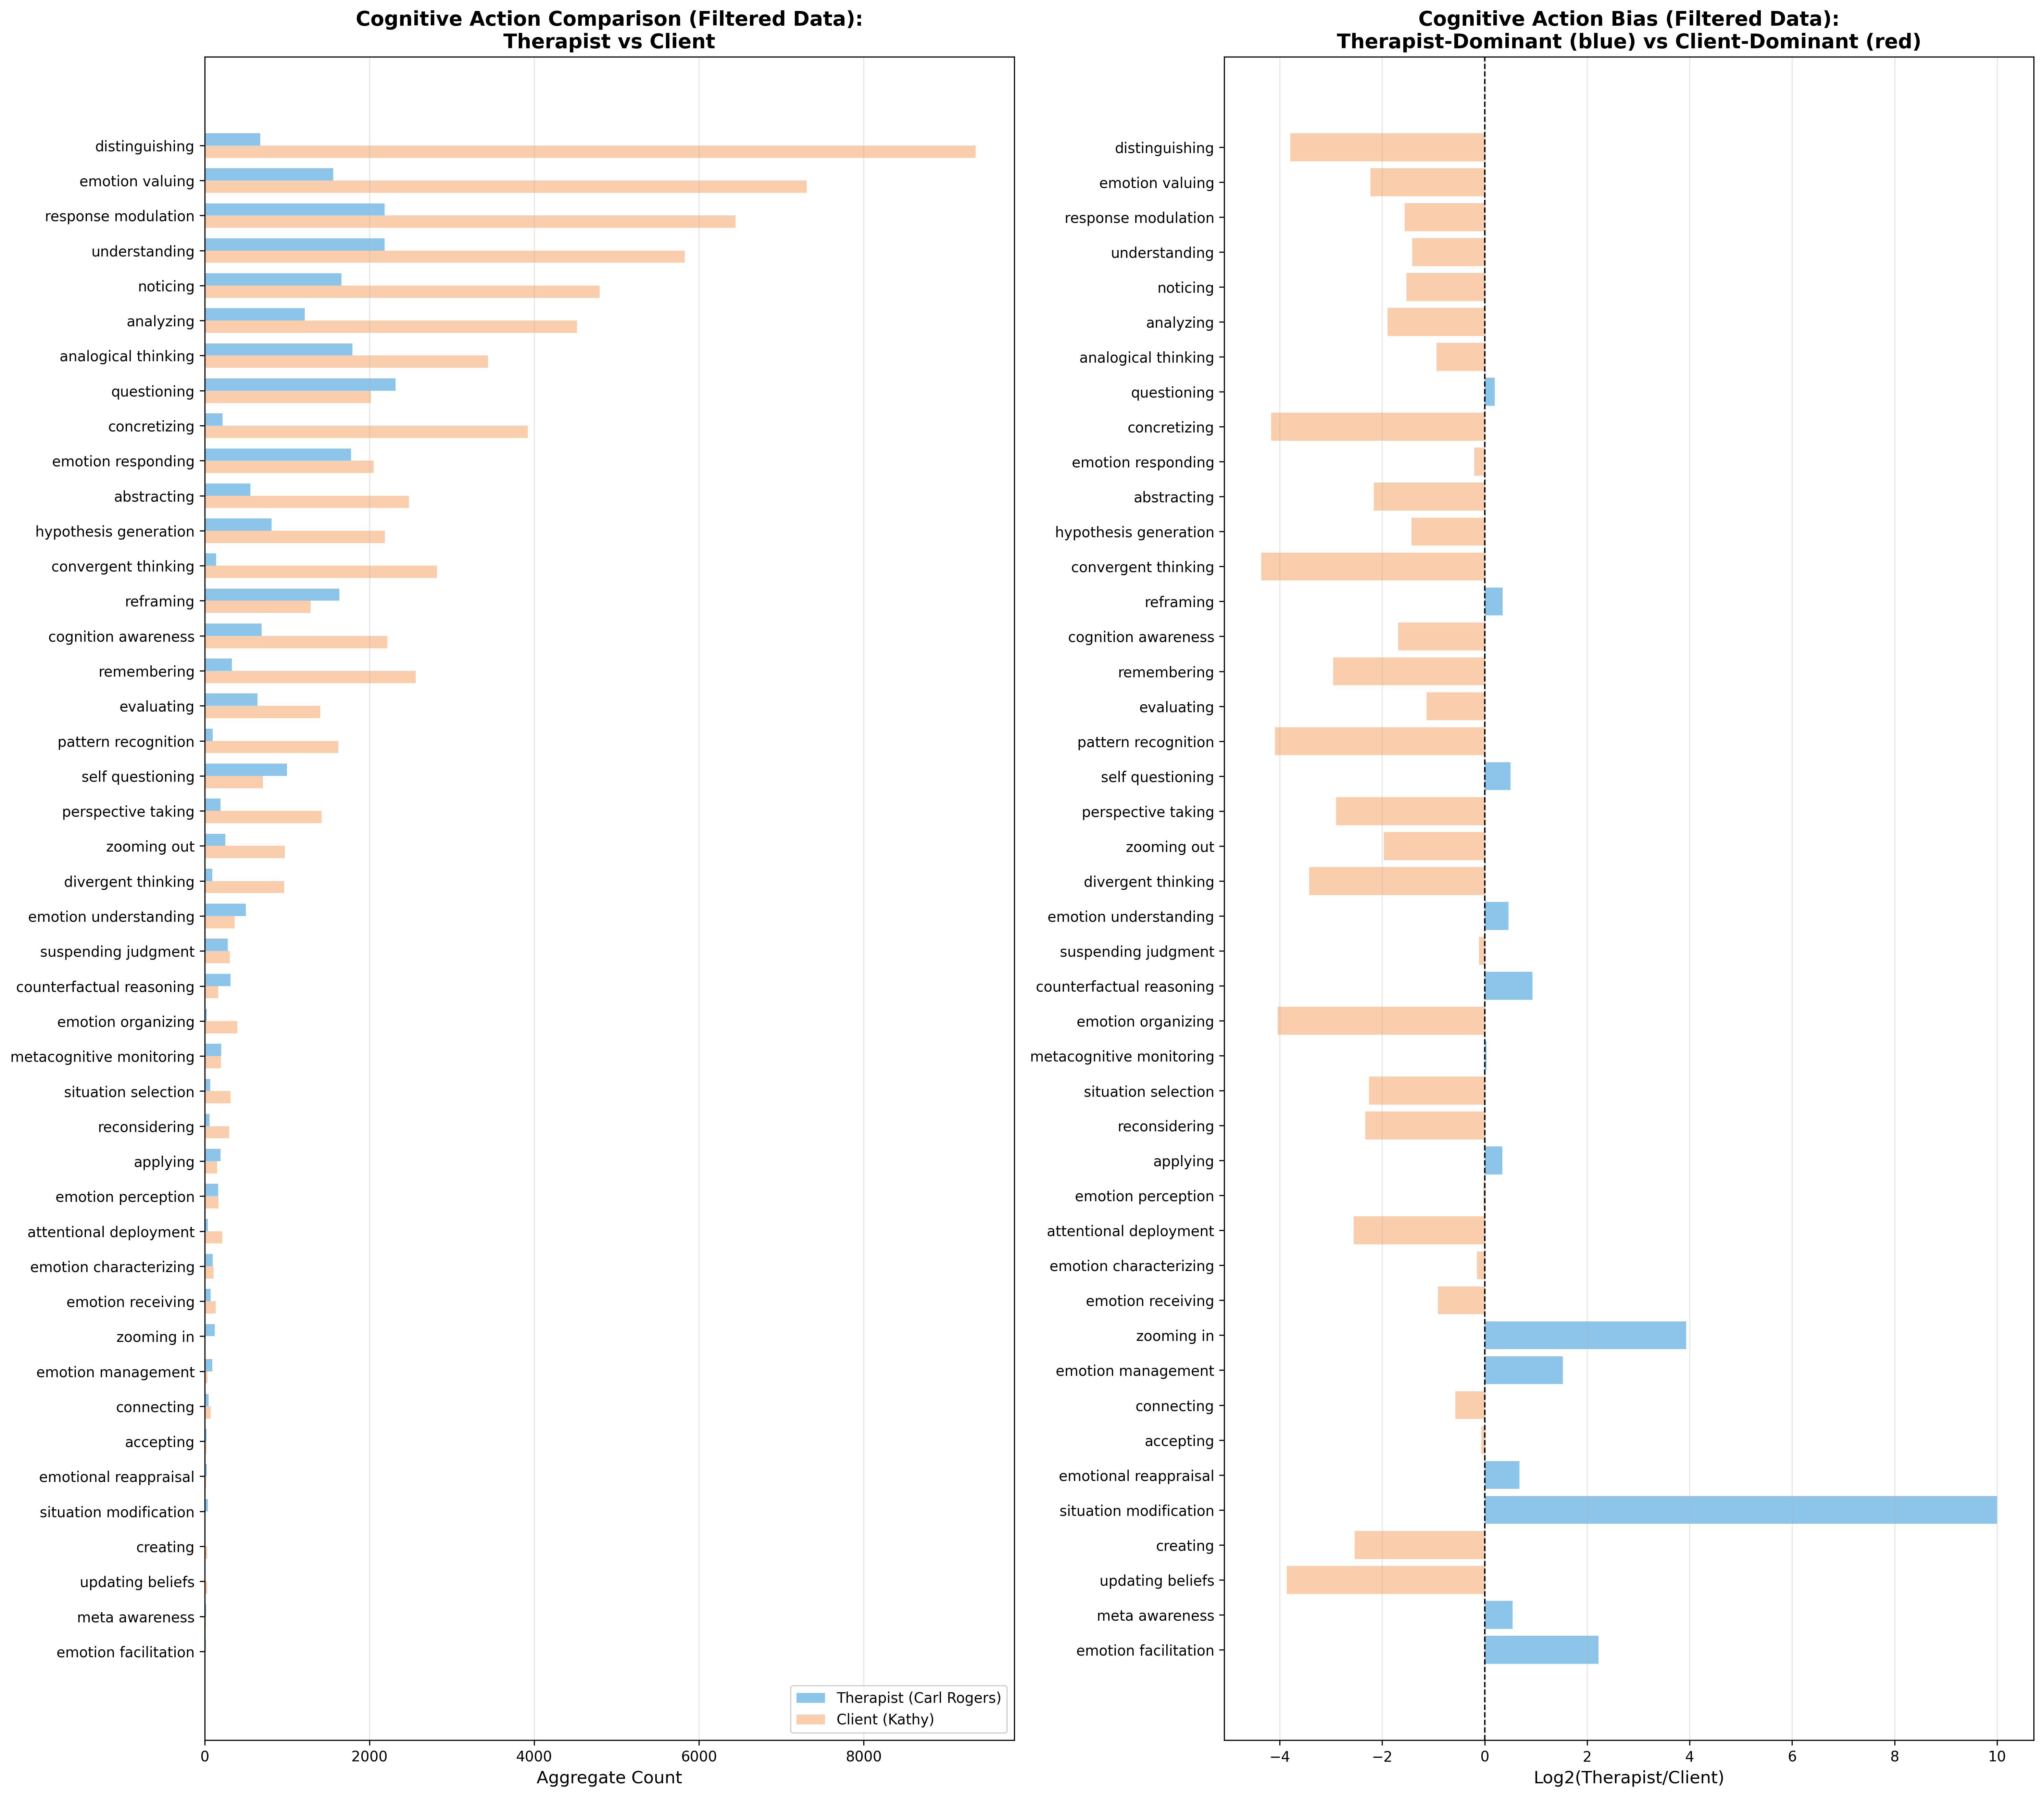
\includegraphics[width=\textwidth]{../Keep_viz/rogers_kathy_comparison.png}
\caption{Cognitive action analysis of Carl Rogers therapy session. Left: Side-by-side comparison of therapist vs client cognitive action frequencies. Right: Log$_2$ ratio showing therapist-dominant (blue) vs client-dominant (red) cognitive patterns. The visualization demonstrates Cogni Map's utility for analyzing therapeutic discourse and identifying role-specific cognitive strategies.}
\label{fig:therapy_viz}
\end{figure*}

\textbf{Visualization 3 - Sentiment Analysis:} Mean sentiment scores (from regression probes trained on layers 1-11, optimal layer 7, R$^2$=0.851) correlate with cognitive actions. Creative actions (Creating: +0.82, Divergent\_thinking: +0.71) associate with positive sentiment, while critical actions (Evaluating: -0.12, Distinguishing: -0.08) are sentiment-neutral, and self-critical actions (Self\_questioning: -0.34) associate with negative sentiment.

\textbf{Clinical Insights:} The detected patterns align with Rogers' theoretical framework where therapists provide "unconditional positive regard" (manifested as Accepting, Perspective\_taking) while clients engage in self-directed change (Reconsidering, Self\_questioning). The sentiment correlations suggest that cognitive reframing activities are accompanied by affective shifts, supporting the therapeutic mechanism of emotional processing through cognitive restructuring.

\subsection{Sentiment Probe Performance}

Our sentiment regression probes achieve strong performance in early-to-mid layers (1-11), with Layer 7 achieving the best results (R$^2$=0.851, MAE=0.308, Accuracy=96.9\%). Figure~\ref{fig:sentiment_performance} shows the dramatic performance degradation after Layer 11, where R$^2$ scores become negative, indicating worse-than-baseline predictions. This suggests that early layers encode sentiment information more directly, while later layers prioritize task-specific representations.

\begin{figure*}[t]
\centering
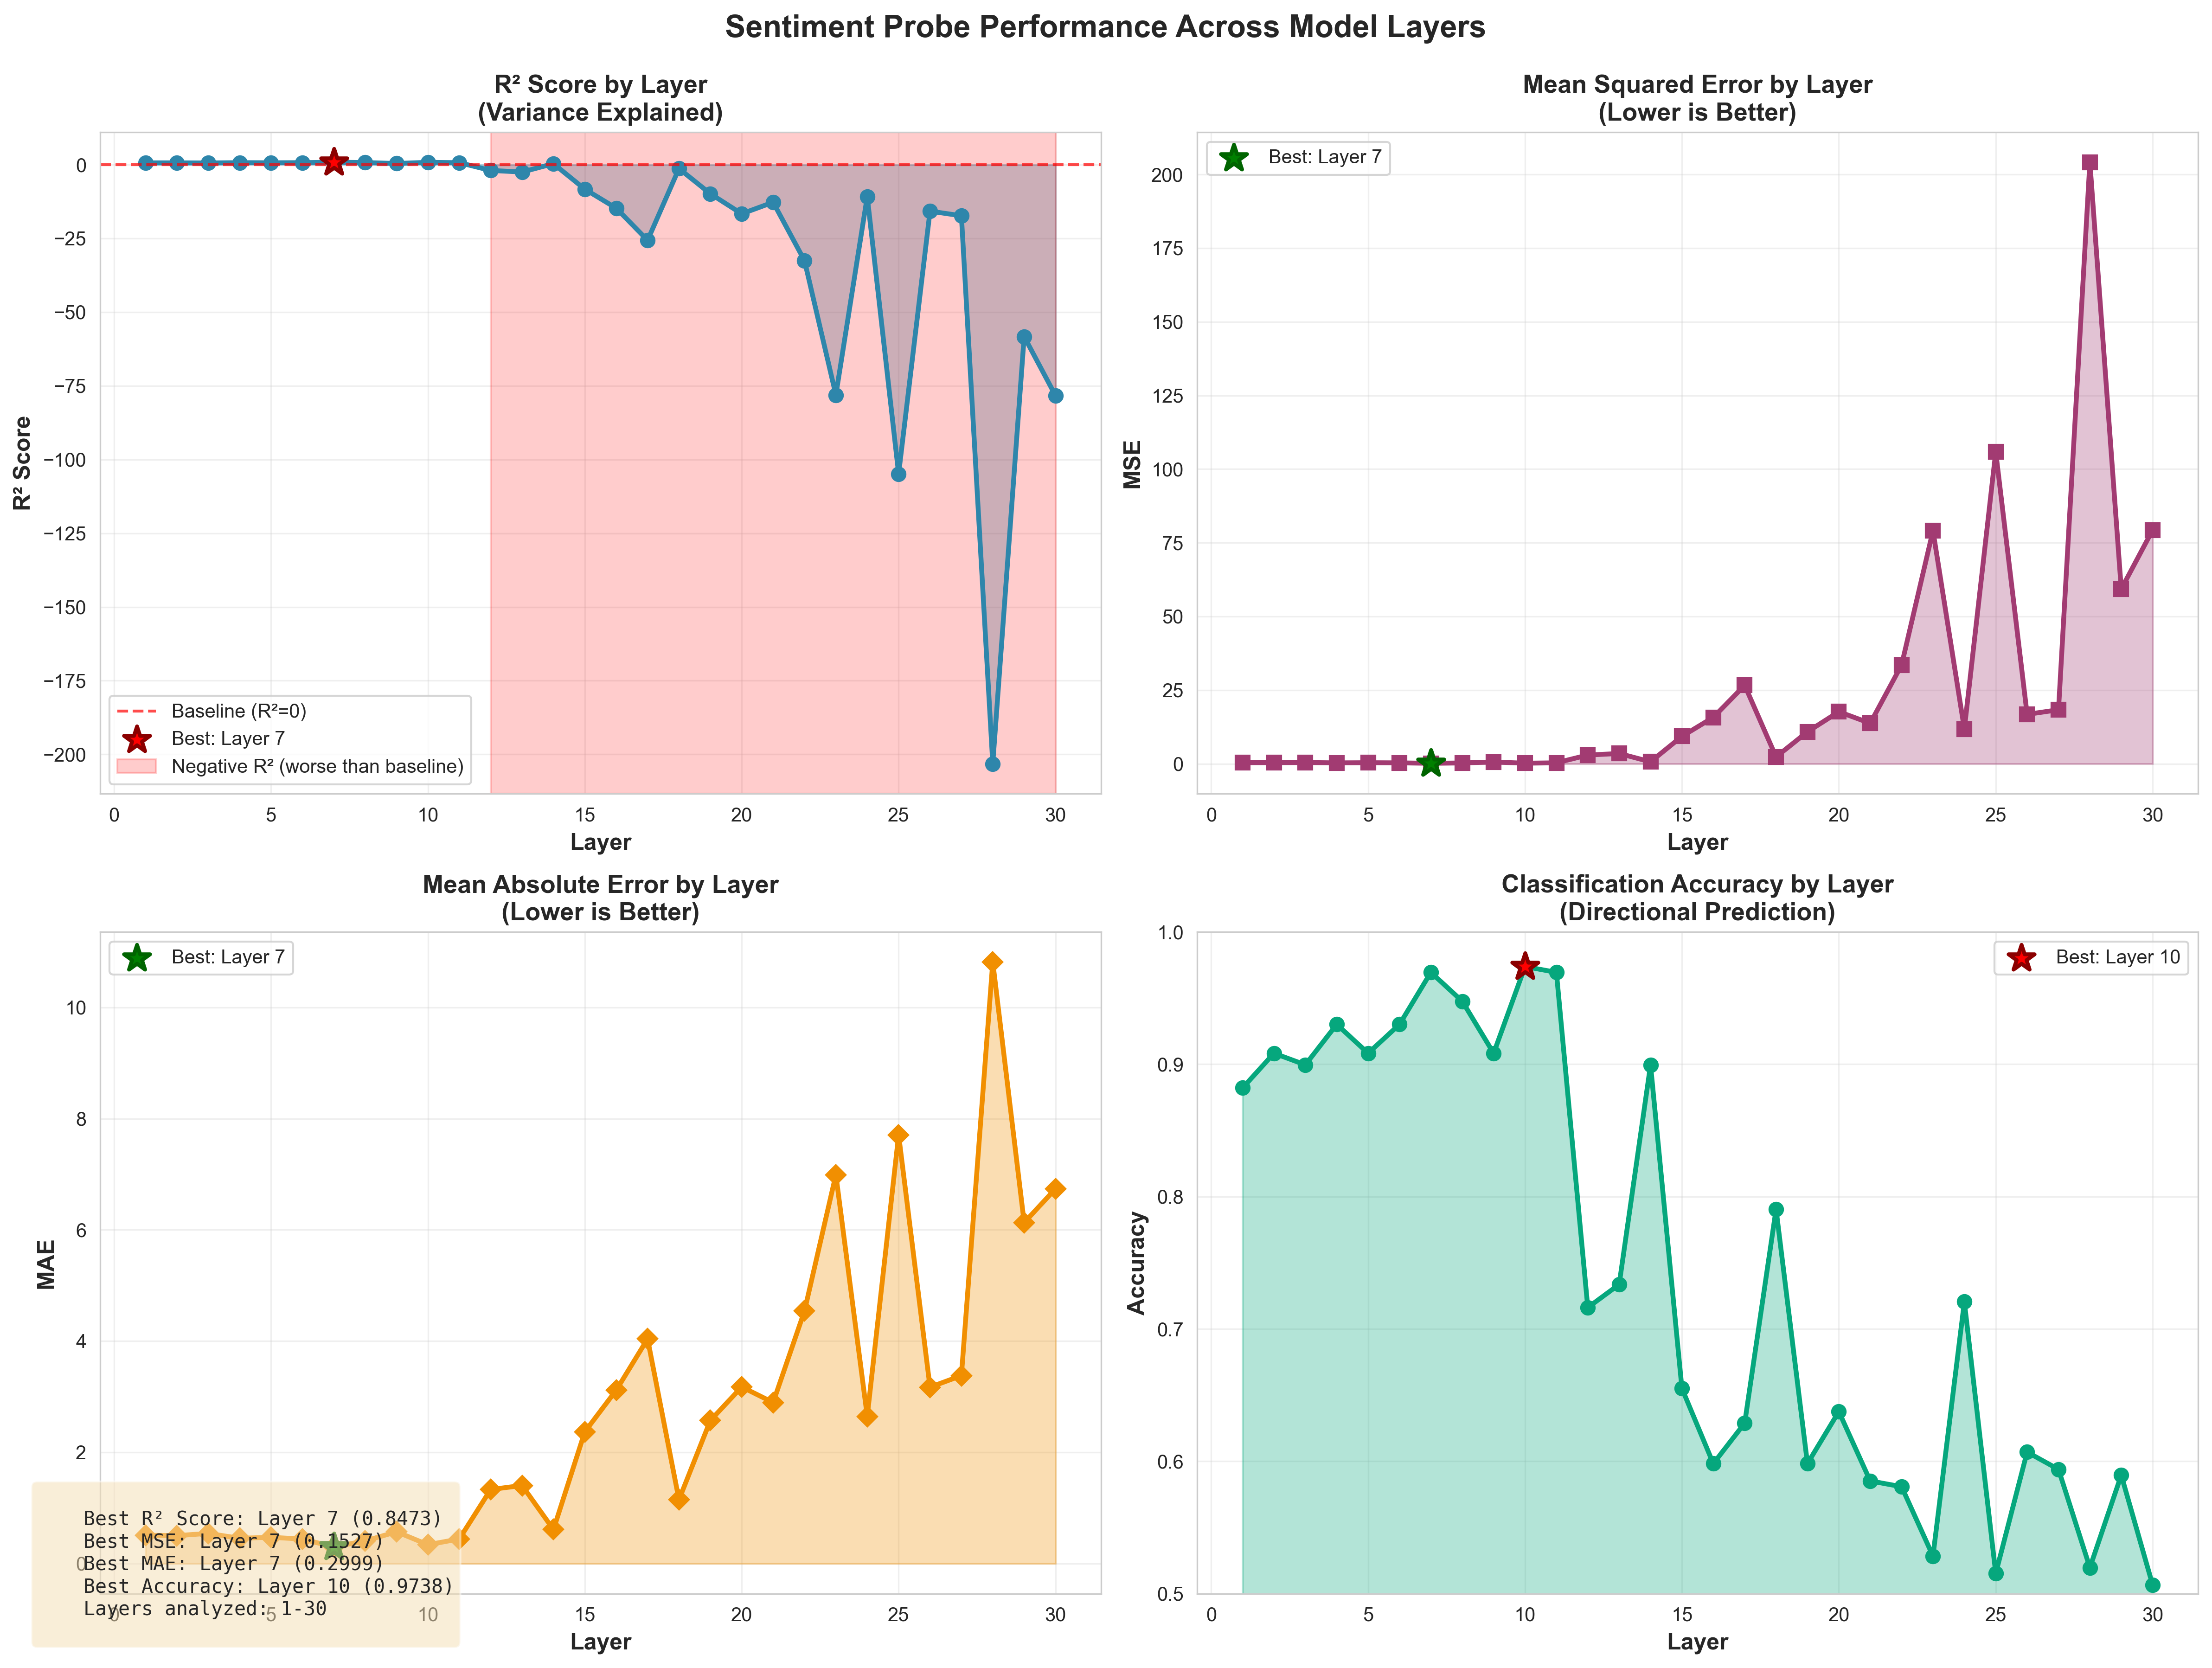
\includegraphics[width=\textwidth]{../data/sentiment_probe_performance.png}
\caption{Sentiment probe performance across all 30 layers. Layer 7 achieves optimal performance (R$^2$=0.851), with a clear performance cliff after Layer 11. Early layers (1-11) show strong sentiment encoding, while later layers show degraded performance with negative R$^2$ values.}
\label{fig:sentiment_performance}
\end{figure*}

\section{Appendix C: Interactive TUI for Qualitative Analysis}

Cogni Map includes a Terminal User Interface (TUI) for qualitative exploration of cognitive actions and sentiment at the token level. Figure~\ref{fig:tui} shows the interface, which provides:

\begin{itemize}
    \item \textbf{Token-level visualization:} Color-coded token streams with activation highlighting
    \item \textbf{Real-time predictions:} Cognitive action and sentiment scores updated per token
    \item \textbf{Layer distribution:} Heatmaps showing which layers activate for each detected action
    \item \textbf{Interactive navigation:} Arrow keys to explore the model's reasoning process dynamically
\end{itemize}

\begin{figure*}[t]
\centering
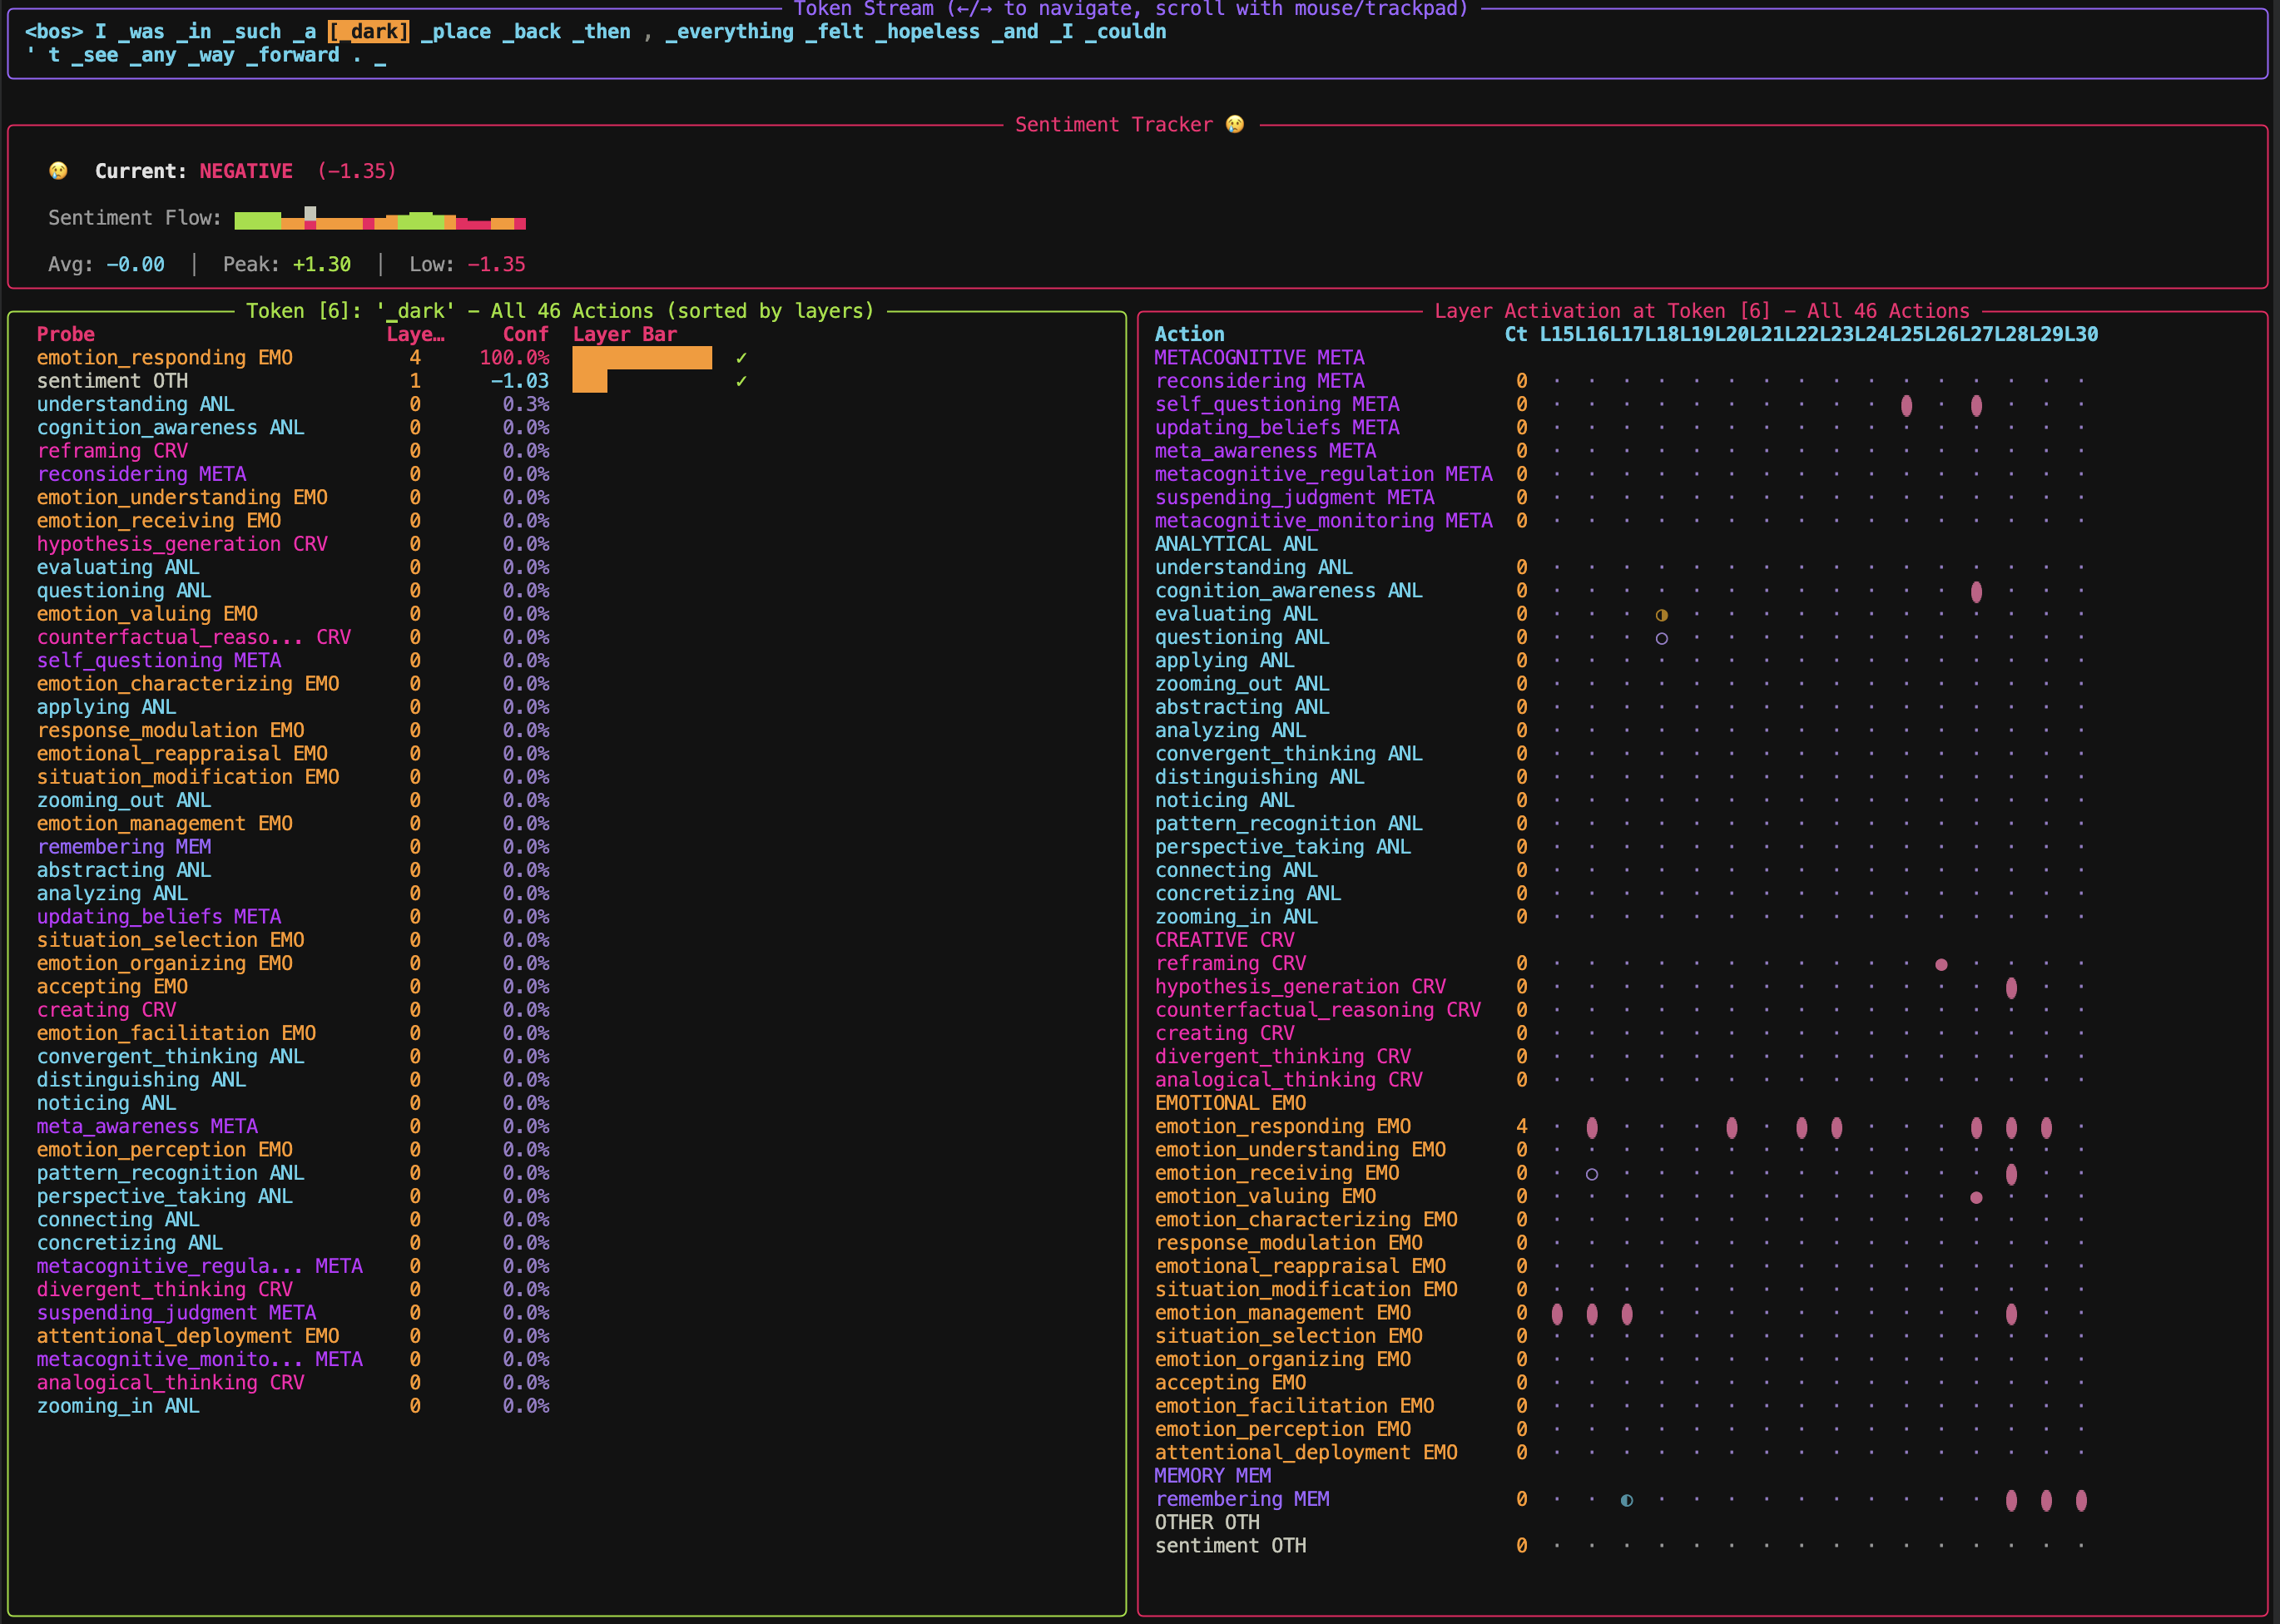
\includegraphics[width=0.9\textwidth]{../data/TUI_example.png}
\caption{Interactive Terminal User Interface (TUI) showing token-level cognitive action detection and sentiment analysis. The interface displays color-coded tokens, real-time predictions, layer-by-layer activation heatmaps, and per-action confidence scores, enabling qualitative exploration of the model's cognitive processes.}
\label{fig:tui}
\end{figure*}

The TUI complements quantitative probe analysis by enabling researchers to interactively explore individual examples, validate probe predictions, and develop intuitions about how cognitive actions manifest at different layers.

\section{Appendix D: Implementation Details}

\textbf{Hardware:} All experiments run on a single NVIDIA A100 GPU (80GB VRAM) with 96GB RAM. Training one linear probe takes $\sim$3 minutes. Activation capture for 31,500 examples (30 layers simultaneously) takes $\sim$2.5 hours.

\textbf{Software:} Python 3.10, PyTorch 2.0, HuggingFace Transformers 4.35, nnsight 0.2 (third-party library for activation intervention).

\textbf{Data Format:} Activations stored in HDF5 format with float32 dtype (converted from bfloat16 for compatibility). Each HDF5 file contains train/val/test groups with `activations` (N × 3072) and `labels` (N,) datasets.

\textbf{Code availability:} Full source code, trained probes, and datasets available at: \texttt{github.com/ChuloIva/Cogni\_map}

\end{document}
